\documentclass[11pt,varwidth=\maxdimen]{standalone}
%\documentclass{article}
\usepackage[english]{babel}	
\usepackage[utf8]{inputenc}	% Allows for writing special charachters in the tex-file 

\usepackage{amsfonts,amsmath,amssymb,bm,mathrsfs,mathtools,dsfont} 	% Standard mathematics 

\usepackage[dvipsnames,table]{xcolor}
\definecolor{rmp}{RGB}{41, 43, 133}
\definecolor{myblue}{rgb}{0.24, 0.36, 0.44}
\definecolor{mygreen}{rgb}{0.367, 0.473, 0.0}
\newcommand{\myBlue}[0]{RoyalBlue}
\newcommand{\myGreen}[0]{OliveGreen}
\newcommand{\myRed}[0]{OrangeRed}
\newcommand{\myYellow}[0]{Goldenrod}


\usepackage{tikz}
\usetikzlibrary{positioning,shapes,calc,arrows.meta}
\newcommand{\coord}[4]{({(#1)+(#3)*cos(#4)},{(#2)+(#3)*sin(#4)})}


\newcommand{\sscript}[1]{{\scriptscriptstyle \mathrm{#1}}}
\newcommand{\EFT}{\sscript{EFT}}


% % % % % % Commands % % % % % % %

\begin{document}

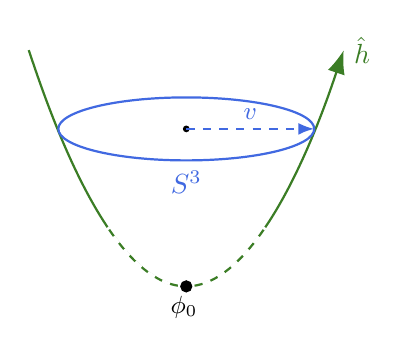
\begin{tikzpicture}
	\tikzset{baseline=(c.base)}
	\node (0,0) (c) {};
	\draw[thick, \myGreen] (0,0) parabola (-2,3);
	\draw[thick, -{Latex[length=3mm]}, \myGreen] (0,0) parabola (2,3) node[right] {$\hat{h}$};
	\draw[very thick, white, dashed] (0,0) parabola (-1,0.75);
	\draw[very thick, white, dashed] (0,0) parabola (+1,0.75);
	\filldraw[black] (0,2) circle (1pt);
	\draw[thick, \myBlue] (0,2) ellipse [x radius=1.625cm,y radius=.4cm] node[below, yshift=-.4cm] {$S^3$};
	\draw[thick, \myBlue, dashed , -{Latex[length=2mm]}] (0,2) -- node[above, yshift=-0.5] {\small $v$} (1.625,2);
	\filldraw[black] (0,0) circle (2pt) node[anchor=north] {\small $\phi_0$\,};
\end{tikzpicture}

\end{document}